\subsubsection{Engstelle}
Anhand dieses Testszenarios soll ermittelt werden, welchen Einfluss das Variieren der Anzahl an Personen im Szenario auf die Simulationsdauer hat. Hierfür müssen die Personen einen $72\ m$ langen und $11,6\ m$ breiten Gang durchlaufen. Nach einer Länge von ca. $68\ m$ befindet sich eine $1,2\ m$ breite und $0,80\ m$ lange Engstelle.
Darüber hinaus wird die Personendichte in einem Messbereich (in den Abildungen rot hervorgehoben) vor der Engstelle gemessen und der Personengeschwindigkeit in einem Fundamentaldiagramm gegenübergestellt. Abbildung \ref{fig:engstelleMAP} zeigt das beschriebene Szenario. Für die Wegefindung wurde in diesem Testszenario der Dijkstra Algorithmus verwendet. 

\begin{figure}
\centering
\begin{minipage}{1\textwidth}
\centering
  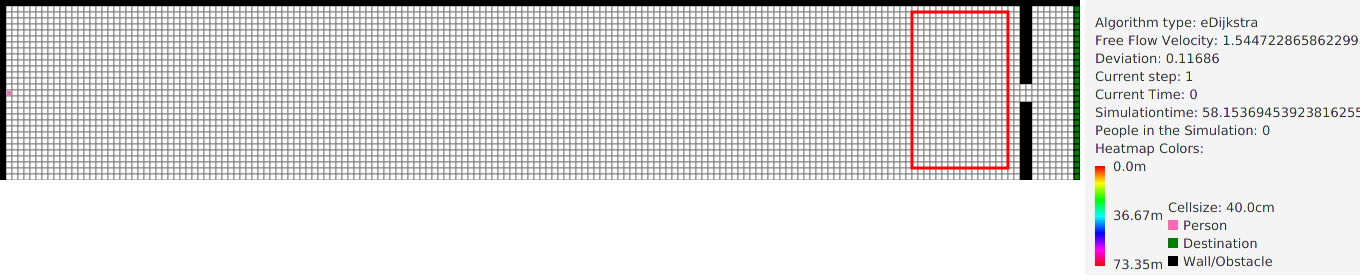
\includegraphics[width=1\linewidth]{abbildungen/engstelle/engstelleMAP.png}
\end{minipage}%
\\
\begin{minipage}{1\textwidth}
\centering
  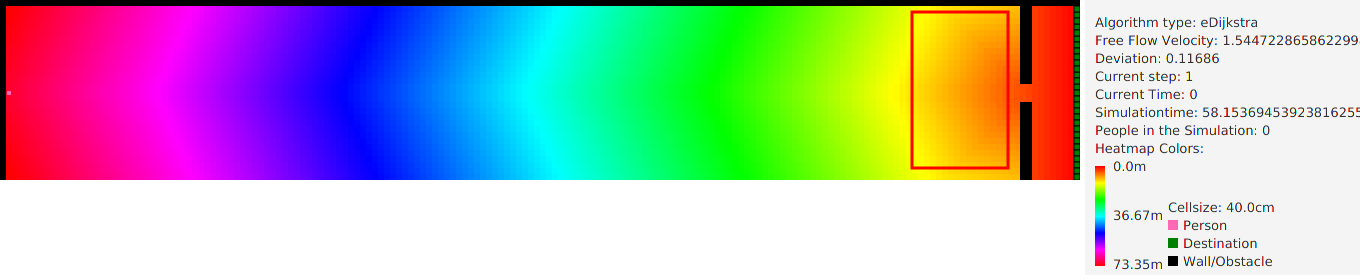
\includegraphics[width=1\linewidth]{abbildungen/engstelle/engstelleHEATMAP.png}
\end{minipage}
\caption{Darstellung der Karte als Cellmap (links) und Heatmap (rechts)}
\label{fig:engstelleMAP}
\end{figure}

Es es wurde zunächst nur eine Person eingefügt, um die Zeit, die für die Überwindung der Strecke benötigt wird zu ermitteln. Anschließend wurde der Test mit 10, 50, 100, 1000 und 2000 Personen wiederholt. Die unterschiedlichen Zeiten sind in der Tabelle \ref{tab:SimuZeitEngstelle} aufgeführt. Bis zu einer Personenzahl von $50$ liegen die Zeiten sehr nah beieinander. Die Simulation zeigt, dass die Anzahl der Personen zu gering bzw. die Engstelle breit genug ist, sodass sich die Personen nicht stauen. Bei einer Personenzahl von $100$ bilden sich erstmals leichte Staus, wodurch die Simulationszeit ($66,82 s$) um ca. $4\ s$ ansteigt.\\

\begin{table}[htpb]
	\centering
	\begin{tabular}{lll}
		Anzahl der Personen & Simulationszeit  &  Besonderheit\\ \hline
		$1$ Person & $58,15\ s$  &  Kein Stau vor der Engstelle\\ 
		$10$ Personen & $59,24\ s$  &  Kein Stau vor der Engstelle\\ 
		$50$ Personen & $62,83\ s$  &  Kein Stau vor der Engstelle\\ 
		$100$ Personen & $66,82\ s$  &  Leichter Stau vor der Engstelle\\ 
		$1000$ Personen & $189,95\ s$  &  Stau vor der Engstelle\\ 
		$2000$ Personen & $329,33\ s$  &  Großer Stau vor der Engstelle\\ 
 
	\end{tabular}
	\caption{Vergleich der unterschiedlichen Simulationszeiten abhängig von der Personenzahl}
	\label{tab:SimuZeitEngstelle}
\end{table}

Die Simulation mit einer Personenzahl von $1000$ zeigt zunächst, dass sich die unterschiedlichen Wunschgeschwindigkeiten der Personen aufgrund des langen Ganges stark auswirken. Schnellere Personen überholen langsamere, sodass nicht alle Personen gleichzeitig die Engstelle erreichen. Trotzdem ist die Anzahl der Personen zu groß bzw. die Engstelle zu schmal, sodass sich die Personen vor der Engstelle stauen. Beides ist in Abbildung \ref{fig:engstelle1000p} zu sehen. Dies wirkt sich deutlich auf die Simulationsdauer aus. Die Personendichte und die Personengeschwindigkeit im Messbereich sind im Fundamentaldiagramm (vgl. Abbildung \ref{fig:engstelle1000pFUNDA} gegenübergestellt. Zusätzlich wurde eine polinomische Trendlinie vierten Grades eingefügt. Im Fundamentaldiagramm ist lediglich der Zeitraum dargestellt, ab dem sich Personen im Messbereich befinden und bis die maximale Dichte erreicht ist. Es ist anzumerken, dass die Verteilung der Personen über den Messbereich nicht gleichmäßig ist. Zu Beginn stauen sich die Personen lediglich in einem Halbkreis um die Engstelle. Wenn die Personen den Messbereich wieder verlassen, also der Stau sich auflöst, verringert sich die Personendichte. Die Geschwindigkeit erhöht sich jedoch nicht signifikant. Dies ist in Abbildung \ref{fig:engstelle1000pFUNDAALL} dargestellt.

\begin{figure}
\centering
\begin{minipage}{1\textwidth}
\centering
  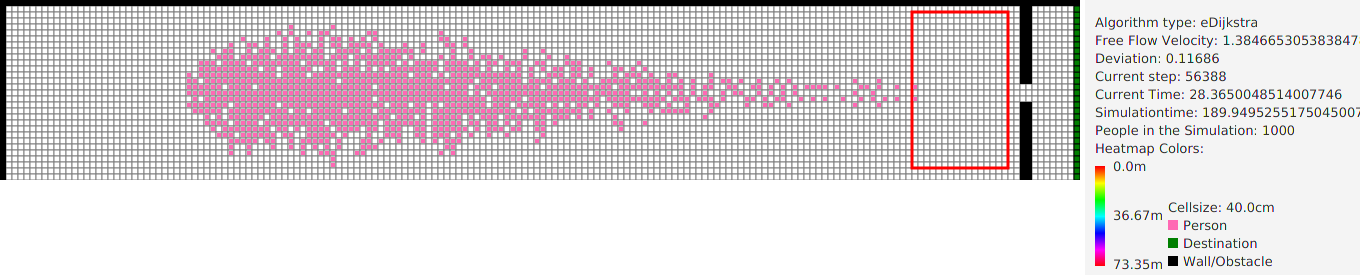
\includegraphics[width=1\linewidth]{abbildungen/engstelle/1000P/engstelle1000personenVORmessbereich.png}
\end{minipage}%
\\
\begin{minipage}{1\textwidth}
\centering
  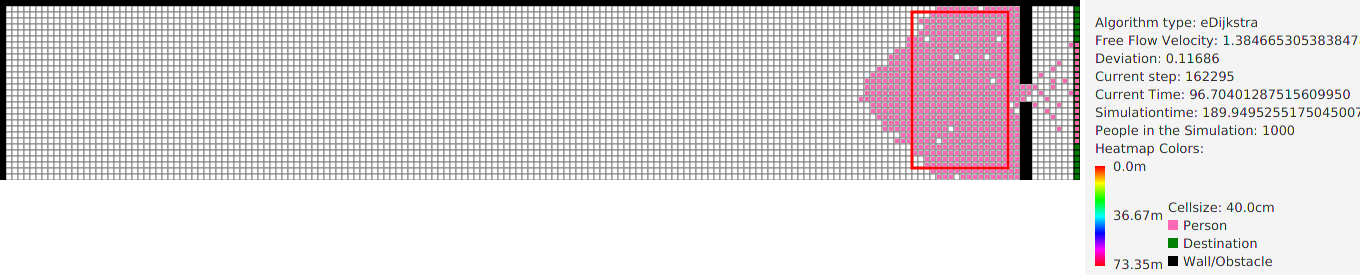
\includegraphics[width=1\linewidth]{abbildungen/engstelle/1000P/engstelle1000personenMAXmessbereich.png} 
 \end{minipage}
\caption{Ausschnitt aus der Simulation mit 1000 Personen, Verteilung der Personen aufgrund individueller Geschwindigkeit (links) und Bildung des Staus vor der Engstelle (rechts)}
\label{fig:engstelle1000p}
\end{figure}

\begin{figure}[ht]
	\centering
  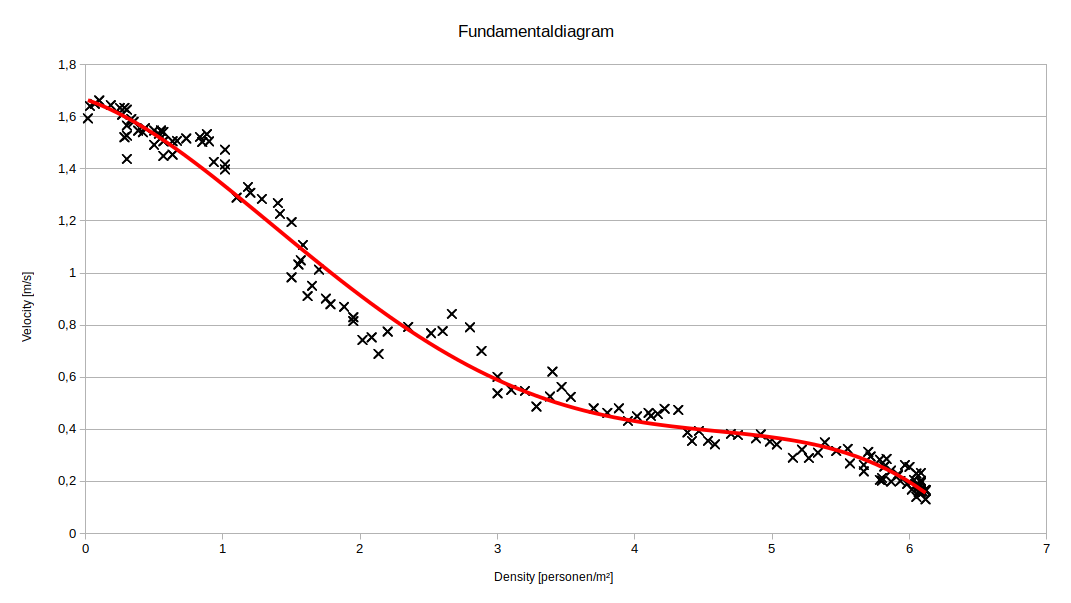
\includegraphics[width=\textwidth]{abbildungen/engstelle/1000P/fundamentalDiagram1000persons.png}
	\caption{Fundamentaldiagramm der Simulation mit 1000 Personen}
	\label{fig:engstelle1000pFUNDA}
\end{figure}

\begin{figure}[ht]
	\centering
  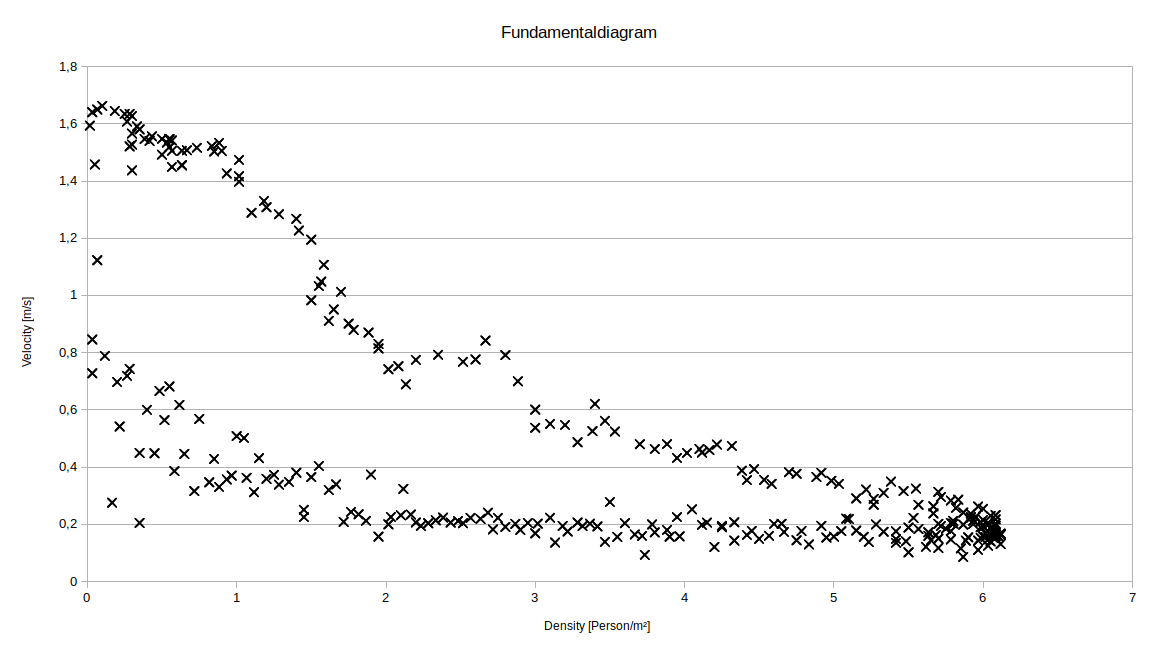
\includegraphics[width=\textwidth]{abbildungen/engstelle/1000P/fundamentalDiagram1000personsALLDATA.png}
	\caption{Fundamentaldiagramm der Simulation mit 1000 Personen (Ab Staubildung bis Ende des Staus)}
	\label{fig:engstelle1000pFUNDAALL}
\end{figure}

Im Vergleich dazu zeigt die Simulation mit 2000 Personen einen deutlichen Stau an der Engstelle. Die Simulationsdauer ist fast doppelt so groß wie bei der Simulation mit 1000 Personen. Die Bewegung der Personen und der Stau vor der Engstelle sind in Abbildung \ref{fig:engstelle2000p} dargestellt. Es wurden ebenfalls zwei Fundamentaldiagramme für den Messbereich erstellt. Abbildung \ref{fig:engstelle2000pFUNDA} zeigt das Fundamentaldiagramm für den Zeitraum zwischen dem ankommen der ersten Person im Messbereich und der maximalen Dichte im Messbereich. Abbildung \ref{fig:engstelle2000pFUNDAALL} zeigt das Fundamentaldiagramm bis zum Zeitpunkt, an dem die letzte Person den Messbereich verlassen hat. Ebenfalls ist zu sehen, dass sich die Geschwindigkeit trotz abnehmender Dichte nicht signifikant erhöht.\\

Zusammenfassend lässt sich feststellen, dass die Engstelle erst ab einer gewissen Personenzahl (in dieser Simulation 100 Personen) überhaupt Auswirkungen auf die Simulationsdauer hat. Bei geringer Personenzahl bleibt die Simulationsdauer annähernd gleich und variiert lediglich aufgrund der normalverteilten Wunschgeschwindigkeit der Personen. 

\begin{figure}
\centering
\begin{minipage}{1\textwidth}
\centering
  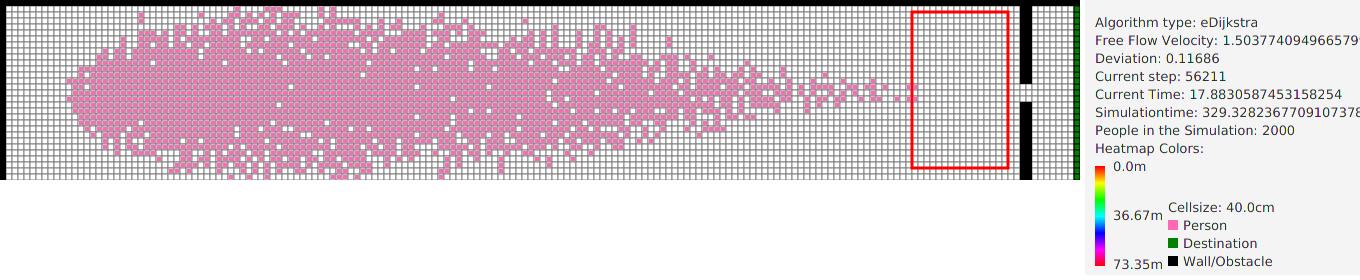
\includegraphics[width=1\linewidth]{abbildungen/engstelle/2000P/engstelle2000personenVORmessbereich.png}
\end{minipage}%
\\
\begin{minipage}{1\textwidth}
\centering
  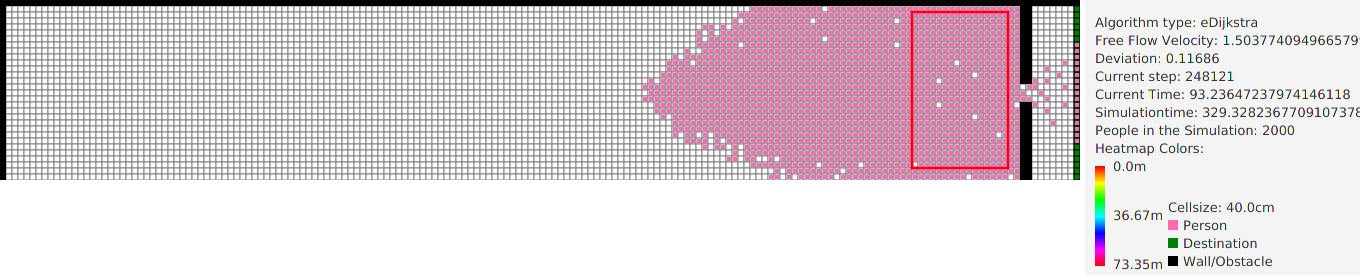
\includegraphics[width=1\linewidth]{abbildungen/engstelle/2000P/engstelle2000personenMAXmessbereich.png} 
 \end{minipage}
\caption{Ausschnitt aus der Simulation mit 2000 Personen, Verteilung der Personen aufgrund individueller Geschwindigkeit (links) und Bildung des Staus vor der Engstelle (rechts)}
\label{fig:engstelle2000p}
\end{figure}

\begin{figure}[ht]
	\centering
  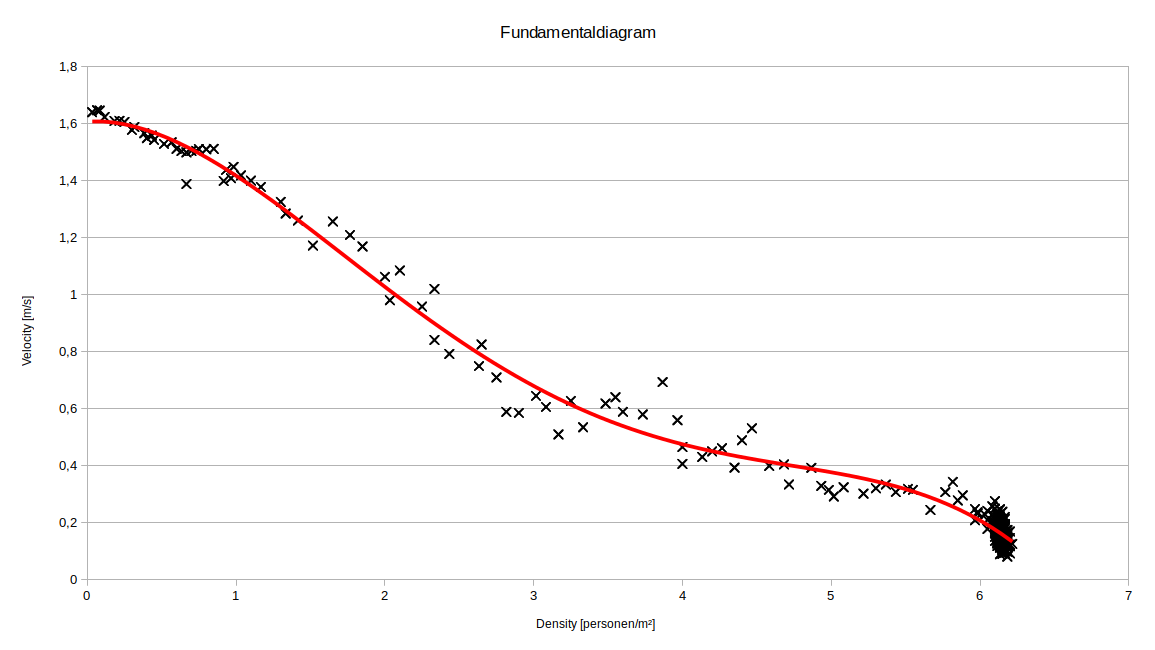
\includegraphics[width=\textwidth]{abbildungen/engstelle/2000P/fundamentalDiagram2000persons.png}
	\caption{Fundamentaldiagramm der Simulation mit 2000 Personen}
	\label{fig:engstelle2000pFUNDA}
\end{figure}

\begin{figure}[ht]
	\centering
  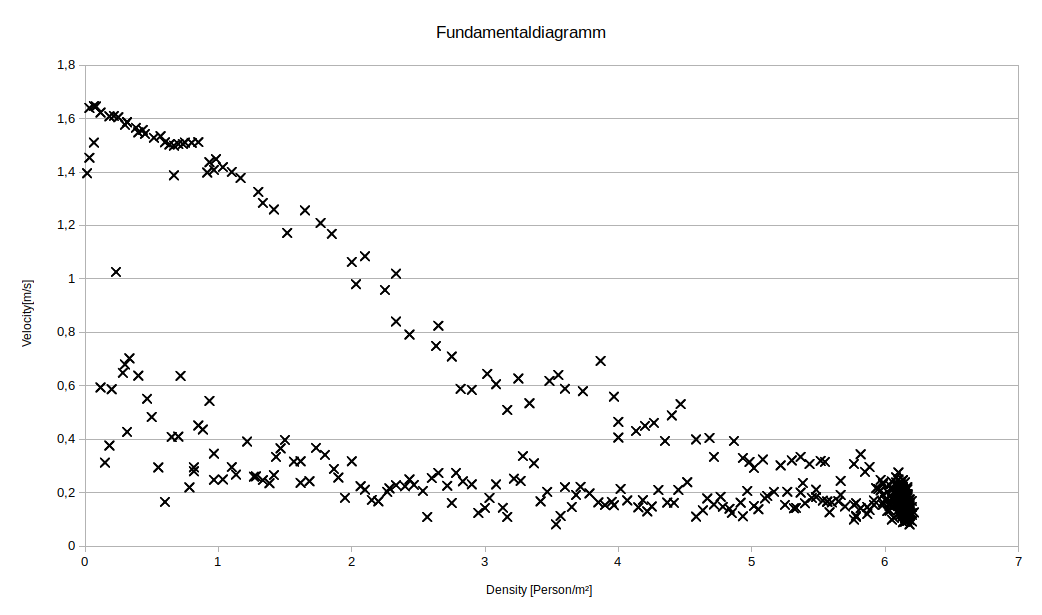
\includegraphics[width=\textwidth]{abbildungen/engstelle/2000P/fundamentalDiagram2000personsALLDATA.png}
	\caption{Fundamentaldiagramm der Simulation mit 2000 Personen (Ab Staubildung bis Ende des Staus)}
	\label{fig:engstelle2000pFUNDAALL}
\end{figure}
